# 局所学習則による最適フィードバック制御
Neural optimal feedback control with local learning rules
システム同定と同時にpolicy gradientを計算する.
\begin{itemize}
\item https://github.com/j-friedrich/neuralOFC/blob/master/ofc.py
\end{itemize}

   
\lstinputlisting[language=julia]{./text/motor-learning/local-learning-ofc/003.jl}
\subsubsection{系の状態変化}


\begin{aligned}
&\text {Dynamics} \quad \mathbf{x}_{t+1}=A \mathbf{x}_{t}+B \mathbf{u}_{t}+\boldsymbol{\xi}_{t}+\sum_{i=1}^{c} \varepsilon_{t}^{i} C_{i} \mathbf{u}_{t}\\
&\text {Feedback} \quad \mathbf{y}_{t}=H \mathbf{x}_{t}+\omega_{t}+\sum_{i=1}^{d} \epsilon_{t}^{i} D_{i} \mathbf{x}_{t}\\
&\text{Cost per step}\quad \mathbf{x}_{t}^\top Q_{t} \mathbf{x}_{t}+\mathbf{u}_{t}^\top R \mathbf{u}_{t}
\end{aligned}


\subsubsection{LQG}
加法ノイズしかない場合($C=D=0$),制御問題は\textbf{\index{せんけい2つぎがうしあん(LQG: linear-quadratic-Gaussian)せいぎょ@線形2次ガウシアン(LQG: linear-quadratic-Gaussian)制御}}と呼ばれる.


\paragraph{運動制御 (Linear-Quadratic Regulator)}


\begin{align}
\mathbf{u}_{t}&=-L_{t} \widehat{\mathbf{x}}_{t}\\
L_{t}&=\left(R+B^{\top} S_{t+1} B\right)^{-1} B^{\top} S_{t+1} A\\
S_{t}&=Q_{t}+A^{\top} S_{t+1}\left(A-B L_{t}\right)\\
s_t &= \mathrm{tr}(S_{t+1}\Omega^\xi) + s_{t+1}; s_T=0
\end{align}


$\boldsymbol{S}_{T}=Q$

\paragraph{状態推定 (Kalman Filter)}


\begin{align}
\widehat{\mathbf{x}}_{t+1}&=A \widehat{\mathbf{x}}_{t}+B \mathbf{u}_{t}+K_{t}\left(\mathbf{y}_{t}-H \widehat{\mathbf{x}}_{t}\right)+\boldsymbol{\eta}_{t} \\ 
K_{t}&=A \Sigma_{t} H^{\top}\left(H \Sigma_{t} H^{\top}+\Omega^{\omega}\right)^{-1} \\ 
\Sigma_{t+1}&=\Omega^{\xi}+\left(A-K_{t} H\right) \Sigma_{t} A^{\top}
\end{align}


この場合に限り,運動制御と状態推定を独立させることができる.
\subsubsection{一般化LQG}
状態および制御依存ノイズがある場合,
\subsection{実装}
ライブラリの読み込みと関数の定義.
\lstinputlisting[language=julia]{./text/motor-learning/local-learning-ofc/007.jl}
\item ToDo: struct 修正 (nが両方に入っている) 
\begin{itemize}
\lstinputlisting[language=julia]{./text/motor-learning/local-learning-ofc/009.jl}
Qの値は各時刻において一般座標 (位置,速度,加速度,躍度)のそれぞれを0にするコストに対する重みづけである.例えば,速度も0にすることを重視すれば2番目の係数を上げる.
$S$と$\Sigma$は各時点での値を一時的にしか必要としないので更新する.
\lstinputlisting[language=julia]{./text/motor-learning/local-learning-ofc/012.jl}
\lstinputlisting[language=julia]{./text/motor-learning/local-learning-ofc/013.jl}
\lstinputlisting[language=julia]{./text/motor-learning/local-learning-ofc/014.jl}
\lstinputlisting[language=julia]{./text/motor-learning/local-learning-ofc/015.jl}
\lstinputlisting[language=julia]{./text/motor-learning/local-learning-ofc/016.jl}
\begin{figure}[ht]
	\centering
	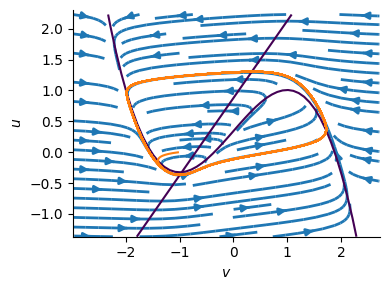
\includegraphics[scale=0.8, max width=\linewidth]{./fig/neuron-model/fhn/cell016.png}
	\caption{cell016.png}
	\label{cell016.png}
\end{figure}
\lstinputlisting[language=julia]{./text/motor-learning/local-learning-ofc/017.jl}
\begin{figure}[ht]
	\centering
	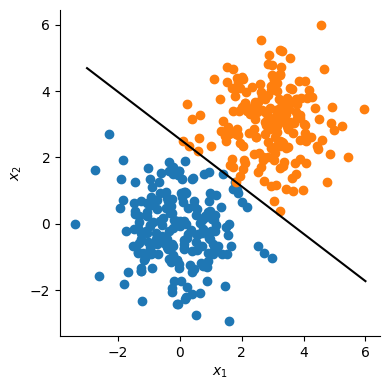
\includegraphics[scale=0.8, max width=\linewidth]{./fig/local-learning-rule/logistic-regression-perceptron/cell017.png}
	\caption{cell017.png}
	\label{cell017.png}
\end{figure}
